% Options for packages loaded elsewhere
% Options for packages loaded elsewhere
\PassOptionsToPackage{unicode}{hyperref}
\PassOptionsToPackage{hyphens}{url}
\PassOptionsToPackage{dvipsnames,svgnames,x11names}{xcolor}
%
\documentclass[
  letterpaper,
  DIV=11,
  numbers=noendperiod]{scrreprt}
\usepackage{xcolor}
\usepackage{amsmath,amssymb}
\setcounter{secnumdepth}{5}
\usepackage{iftex}
\ifPDFTeX
  \usepackage[T1]{fontenc}
  \usepackage[utf8]{inputenc}
  \usepackage{textcomp} % provide euro and other symbols
\else % if luatex or xetex
  \usepackage{unicode-math} % this also loads fontspec
  \defaultfontfeatures{Scale=MatchLowercase}
  \defaultfontfeatures[\rmfamily]{Ligatures=TeX,Scale=1}
\fi
\usepackage{lmodern}
\ifPDFTeX\else
  % xetex/luatex font selection
\fi
% Use upquote if available, for straight quotes in verbatim environments
\IfFileExists{upquote.sty}{\usepackage{upquote}}{}
\IfFileExists{microtype.sty}{% use microtype if available
  \usepackage[]{microtype}
  \UseMicrotypeSet[protrusion]{basicmath} % disable protrusion for tt fonts
}{}
\makeatletter
\@ifundefined{KOMAClassName}{% if non-KOMA class
  \IfFileExists{parskip.sty}{%
    \usepackage{parskip}
  }{% else
    \setlength{\parindent}{0pt}
    \setlength{\parskip}{6pt plus 2pt minus 1pt}}
}{% if KOMA class
  \KOMAoptions{parskip=half}}
\makeatother
% Make \paragraph and \subparagraph free-standing
\makeatletter
\ifx\paragraph\undefined\else
  \let\oldparagraph\paragraph
  \renewcommand{\paragraph}{
    \@ifstar
      \xxxParagraphStar
      \xxxParagraphNoStar
  }
  \newcommand{\xxxParagraphStar}[1]{\oldparagraph*{#1}\mbox{}}
  \newcommand{\xxxParagraphNoStar}[1]{\oldparagraph{#1}\mbox{}}
\fi
\ifx\subparagraph\undefined\else
  \let\oldsubparagraph\subparagraph
  \renewcommand{\subparagraph}{
    \@ifstar
      \xxxSubParagraphStar
      \xxxSubParagraphNoStar
  }
  \newcommand{\xxxSubParagraphStar}[1]{\oldsubparagraph*{#1}\mbox{}}
  \newcommand{\xxxSubParagraphNoStar}[1]{\oldsubparagraph{#1}\mbox{}}
\fi
\makeatother

\usepackage{color}
\usepackage{fancyvrb}
\newcommand{\VerbBar}{|}
\newcommand{\VERB}{\Verb[commandchars=\\\{\}]}
\DefineVerbatimEnvironment{Highlighting}{Verbatim}{commandchars=\\\{\}}
% Add ',fontsize=\small' for more characters per line
\usepackage{framed}
\definecolor{shadecolor}{RGB}{241,243,245}
\newenvironment{Shaded}{\begin{snugshade}}{\end{snugshade}}
\newcommand{\AlertTok}[1]{\textcolor[rgb]{0.68,0.00,0.00}{#1}}
\newcommand{\AnnotationTok}[1]{\textcolor[rgb]{0.37,0.37,0.37}{#1}}
\newcommand{\AttributeTok}[1]{\textcolor[rgb]{0.40,0.45,0.13}{#1}}
\newcommand{\BaseNTok}[1]{\textcolor[rgb]{0.68,0.00,0.00}{#1}}
\newcommand{\BuiltInTok}[1]{\textcolor[rgb]{0.00,0.23,0.31}{#1}}
\newcommand{\CharTok}[1]{\textcolor[rgb]{0.13,0.47,0.30}{#1}}
\newcommand{\CommentTok}[1]{\textcolor[rgb]{0.37,0.37,0.37}{#1}}
\newcommand{\CommentVarTok}[1]{\textcolor[rgb]{0.37,0.37,0.37}{\textit{#1}}}
\newcommand{\ConstantTok}[1]{\textcolor[rgb]{0.56,0.35,0.01}{#1}}
\newcommand{\ControlFlowTok}[1]{\textcolor[rgb]{0.00,0.23,0.31}{\textbf{#1}}}
\newcommand{\DataTypeTok}[1]{\textcolor[rgb]{0.68,0.00,0.00}{#1}}
\newcommand{\DecValTok}[1]{\textcolor[rgb]{0.68,0.00,0.00}{#1}}
\newcommand{\DocumentationTok}[1]{\textcolor[rgb]{0.37,0.37,0.37}{\textit{#1}}}
\newcommand{\ErrorTok}[1]{\textcolor[rgb]{0.68,0.00,0.00}{#1}}
\newcommand{\ExtensionTok}[1]{\textcolor[rgb]{0.00,0.23,0.31}{#1}}
\newcommand{\FloatTok}[1]{\textcolor[rgb]{0.68,0.00,0.00}{#1}}
\newcommand{\FunctionTok}[1]{\textcolor[rgb]{0.28,0.35,0.67}{#1}}
\newcommand{\ImportTok}[1]{\textcolor[rgb]{0.00,0.46,0.62}{#1}}
\newcommand{\InformationTok}[1]{\textcolor[rgb]{0.37,0.37,0.37}{#1}}
\newcommand{\KeywordTok}[1]{\textcolor[rgb]{0.00,0.23,0.31}{\textbf{#1}}}
\newcommand{\NormalTok}[1]{\textcolor[rgb]{0.00,0.23,0.31}{#1}}
\newcommand{\OperatorTok}[1]{\textcolor[rgb]{0.37,0.37,0.37}{#1}}
\newcommand{\OtherTok}[1]{\textcolor[rgb]{0.00,0.23,0.31}{#1}}
\newcommand{\PreprocessorTok}[1]{\textcolor[rgb]{0.68,0.00,0.00}{#1}}
\newcommand{\RegionMarkerTok}[1]{\textcolor[rgb]{0.00,0.23,0.31}{#1}}
\newcommand{\SpecialCharTok}[1]{\textcolor[rgb]{0.37,0.37,0.37}{#1}}
\newcommand{\SpecialStringTok}[1]{\textcolor[rgb]{0.13,0.47,0.30}{#1}}
\newcommand{\StringTok}[1]{\textcolor[rgb]{0.13,0.47,0.30}{#1}}
\newcommand{\VariableTok}[1]{\textcolor[rgb]{0.07,0.07,0.07}{#1}}
\newcommand{\VerbatimStringTok}[1]{\textcolor[rgb]{0.13,0.47,0.30}{#1}}
\newcommand{\WarningTok}[1]{\textcolor[rgb]{0.37,0.37,0.37}{\textit{#1}}}

\usepackage{longtable,booktabs,array}
\usepackage{calc} % for calculating minipage widths
% Correct order of tables after \paragraph or \subparagraph
\usepackage{etoolbox}
\makeatletter
\patchcmd\longtable{\par}{\if@noskipsec\mbox{}\fi\par}{}{}
\makeatother
% Allow footnotes in longtable head/foot
\IfFileExists{footnotehyper.sty}{\usepackage{footnotehyper}}{\usepackage{footnote}}
\makesavenoteenv{longtable}
\usepackage{graphicx}
\makeatletter
\newsavebox\pandoc@box
\newcommand*\pandocbounded[1]{% scales image to fit in text height/width
  \sbox\pandoc@box{#1}%
  \Gscale@div\@tempa{\textheight}{\dimexpr\ht\pandoc@box+\dp\pandoc@box\relax}%
  \Gscale@div\@tempb{\linewidth}{\wd\pandoc@box}%
  \ifdim\@tempb\p@<\@tempa\p@\let\@tempa\@tempb\fi% select the smaller of both
  \ifdim\@tempa\p@<\p@\scalebox{\@tempa}{\usebox\pandoc@box}%
  \else\usebox{\pandoc@box}%
  \fi%
}
% Set default figure placement to htbp
\def\fps@figure{htbp}
\makeatother





\setlength{\emergencystretch}{3em} % prevent overfull lines

\providecommand{\tightlist}{%
  \setlength{\itemsep}{0pt}\setlength{\parskip}{0pt}}



 


\KOMAoption{captions}{tableheading}
\makeatletter
\@ifpackageloaded{tcolorbox}{}{\usepackage[skins,breakable]{tcolorbox}}
\@ifpackageloaded{fontawesome5}{}{\usepackage{fontawesome5}}
\definecolor{quarto-callout-color}{HTML}{909090}
\definecolor{quarto-callout-note-color}{HTML}{0758E5}
\definecolor{quarto-callout-important-color}{HTML}{CC1914}
\definecolor{quarto-callout-warning-color}{HTML}{EB9113}
\definecolor{quarto-callout-tip-color}{HTML}{00A047}
\definecolor{quarto-callout-caution-color}{HTML}{FC5300}
\definecolor{quarto-callout-color-frame}{HTML}{acacac}
\definecolor{quarto-callout-note-color-frame}{HTML}{4582ec}
\definecolor{quarto-callout-important-color-frame}{HTML}{d9534f}
\definecolor{quarto-callout-warning-color-frame}{HTML}{f0ad4e}
\definecolor{quarto-callout-tip-color-frame}{HTML}{02b875}
\definecolor{quarto-callout-caution-color-frame}{HTML}{fd7e14}
\makeatother
\makeatletter
\@ifpackageloaded{bookmark}{}{\usepackage{bookmark}}
\makeatother
\makeatletter
\@ifpackageloaded{caption}{}{\usepackage{caption}}
\AtBeginDocument{%
\ifdefined\contentsname
  \renewcommand*\contentsname{Table of contents}
\else
  \newcommand\contentsname{Table of contents}
\fi
\ifdefined\listfigurename
  \renewcommand*\listfigurename{List of Figures}
\else
  \newcommand\listfigurename{List of Figures}
\fi
\ifdefined\listtablename
  \renewcommand*\listtablename{List of Tables}
\else
  \newcommand\listtablename{List of Tables}
\fi
\ifdefined\figurename
  \renewcommand*\figurename{Figure}
\else
  \newcommand\figurename{Figure}
\fi
\ifdefined\tablename
  \renewcommand*\tablename{Table}
\else
  \newcommand\tablename{Table}
\fi
}
\@ifpackageloaded{float}{}{\usepackage{float}}
\floatstyle{ruled}
\@ifundefined{c@chapter}{\newfloat{codelisting}{h}{lop}}{\newfloat{codelisting}{h}{lop}[chapter]}
\floatname{codelisting}{Listing}
\newcommand*\listoflistings{\listof{codelisting}{List of Listings}}
\makeatother
\makeatletter
\makeatother
\makeatletter
\@ifpackageloaded{caption}{}{\usepackage{caption}}
\@ifpackageloaded{subcaption}{}{\usepackage{subcaption}}
\makeatother
\usepackage{bookmark}
\IfFileExists{xurl.sty}{\usepackage{xurl}}{} % add URL line breaks if available
\urlstyle{same}
\hypersetup{
  pdftitle={VMRDH-Jobs},
  pdfauthor={Document-ID: ?env:git\_hash},
  colorlinks=true,
  linkcolor={blue},
  filecolor={Maroon},
  citecolor={Blue},
  urlcolor={Blue},
  pdfcreator={LaTeX via pandoc}}


\title{VMRDH-Jobs}
\author{Document-ID: \textbf{?env:git\_hash}}
\date{2025-05-19}
\begin{document}
\maketitle

\renewcommand*\contentsname{Job index}
{
\hypersetup{linkcolor=blue}
\setcounter{tocdepth}{2}
\tableofcontents
}

\bookmarksetup{startatroot}

\chapter*{VMRDH 3.0}\label{vmrdh-3.0}
\addcontentsline{toc}{chapter}{VMRDH 3.0}

\markboth{VMRDH 3.0}{VMRDH 3.0}

This pdf acts as a manual to understand the OmniTrans jobs, their
purpose, inputs and outputs.It also allows you to download the jobs and
input templates.

\part{Standard Uitvoer}

\chapter{Matrix Compressies}\label{matrix-compressies}

\section{Purpose}

There are 4 types of matrix compression jobs. Each job has a different
spatial aggregation level. The four aggregation levels are :

\begin{itemize}
\tightlist
\item
  Stedelijkheid
\item
  Gemeenten
\item
  MRDH groot / MRDH groot etm
\item
  MRDH Studiegebied
\end{itemize}

\pandocbounded{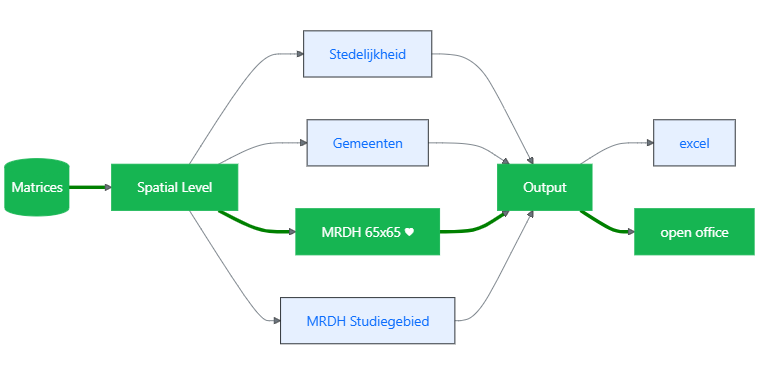
\includegraphics[keepaspectratio]{images/compression.png}}

\begin{verbatim}
\end{verbatim}

\section{Inputs}

The inputs for the job are matrices listed under \texttt{\$matrices}.
Different jobs handle the different level of aggregation for you, so you
do not have to change anything else in the job (see outputs if you want
to change output formats). The input \texttt{\$matrices}takes a list,
each item in the list takes the form
\texttt{{[}"Output\_Sheet\_name",\ {[}P,M,T,U{]}{]},}.

\begin{tcolorbox}[enhanced jigsaw, bottomtitle=1mm, title=\textcolor{quarto-callout-important-color}{\faExclamation}\hspace{0.5em}{Important}, rightrule=.15mm, toptitle=1mm, colbacktitle=quarto-callout-important-color!10!white, opacitybacktitle=0.6, leftrule=.75mm, opacityback=0, coltitle=black, colframe=quarto-callout-important-color-frame, toprule=.15mm, titlerule=0mm, breakable, bottomrule=.15mm, arc=.35mm, colback=white, left=2mm]

Each spatial level is a different job. If you have changed only the list
of matrices in the job, you can use it without caution. But if you have
changed the \texttt{\#\ definieer\ Gebieden} part of the code, that is,
if you have changed the definition of each gebied, you have to be
careful that each \emph{Centroid Number} is exclusively in ONLY ONE
\emph{gebied}. If not, you will get an error.

\end{tcolorbox}

\section{Outputs}

You also have to control the output format. The output can be in two
formats: excel or openoffice. If you are working on the MRDH servers,
you must open/ uncomment the \texttt{Naar\ Open\ Office} and the the two
lines below it. If you want to get an excel format output, you would
comment the \texttt{Naar\ Open\ Office} and the the two lines below it
and uncomment \texttt{Naar\ Excel} and the two lines below it.

\section{Code}

Download the code.\href{../first.rb}{matrixcompress.rb}

\chapter{Voertuigprestaties}\label{voertuigprestaties}

\section{Purpose}

The voertuigprestaties ( or vehicle-km, vehicle-hours) is a performance
indicator for the whole network (or selected-part of a network). This
indicator shows how many km were travelled by all the vehicles
collectively in the network or how many hours were spent by all the
vehicles collectively in the network. More time spent by vehicles in the
network could indicate congestion. Similarly more vehicle-km driven by
vehicles indicate higher pollution/ fuel-usage levels for example.

\section{Inputs}

\begin{tcolorbox}[enhanced jigsaw, bottomtitle=1mm, title=\textcolor{quarto-callout-important-color}{\faExclamation}\hspace{0.5em}{Important}, rightrule=.15mm, toptitle=1mm, colbacktitle=quarto-callout-important-color!10!white, opacitybacktitle=0.6, leftrule=.75mm, opacityback=0, coltitle=black, colframe=quarto-callout-important-color-frame, toprule=.15mm, titlerule=0mm, breakable, bottomrule=.15mm, arc=.35mm, colback=white, left=2mm]

Be careful! Each line of this job is an input parameter. Read carefully
and select the pmturi numbers very carefully.

\end{tcolorbox}

\begin{itemize}
\item
  \texttt{vgtm.load}: In this parameter, you create a list {[}{]}. Each
  item in the list is a pmturi and enclosed inside {[}{]}. Each item is
  separated by a comma.
\item
  \texttt{vgtm.netwerk} : In this parameter, you create a list {[}{]}.
  Each item in the list is a p and m combination refereing to a network.
  The number of items in this list should be same as the number of items
  in \texttt{vgtm.load}.
\item
  \texttt{vgtm.loadNaam} : In this parameter you create a list {[}{]}.
  Each item in this list is a string that defines the name of the load
  defined under \texttt{vgtm.load}. The number of items in this list
  should be same as the number of items in \texttt{vgtm.load}.
\item
  \texttt{vtgkm.variant}: This parameter is also a list {[}{]} and
  contains items that are names of the variants in your model. It is not
  necessary that the number of items in this list is same as number of
  items in the \texttt{vgtm.load}.
\item
  \texttt{vtgkm.selectie} : If you want to calculate these performance
  indictors only for a small part of the network, you must first define
  a selection in omnitrans, give it a name. In this job, you refer to
  that name in this parameter. Again, this parameters is a list and can
  take multiple \texttt{selection-names}.
\item
  \texttt{vtgkm.wegtype} : You have this optional parameter to calculate
  this indicator only for certain wegtypes. This parameter is again a
  list of items indicating the wegtype.
\item
  \texttt{vtgkm.filterWegtype}: You have this optional parameter that a
  list of wegtypes. For example you want to calculate the indicator for
  all links but not connectors. Then you must exclude the connector
  wegtype in this list.
\end{itemize}

\begin{Shaded}
\begin{Highlighting}[]

\CommentTok{\#\# pmturi load}
\NormalTok{vtgkm}\AttributeTok{.load}          \OperatorTok{=} \KeywordTok{[} \KeywordTok{[}\DecValTok{1}\NormalTok{,}\DecValTok{2}\NormalTok{,}\DecValTok{1}\NormalTok{,}\DecValTok{103}\NormalTok{,}\DecValTok{11}\NormalTok{,}\DecValTok{20}\KeywordTok{]}\NormalTok{,}\KeywordTok{[}\DecValTok{1}\NormalTok{,}\DecValTok{2}\NormalTok{,}\DecValTok{3}\NormalTok{,}\DecValTok{103}\NormalTok{,}\DecValTok{11}\NormalTok{,}\DecValTok{20}\KeywordTok{]]}\CommentTok{\# verplicht!}

\CommentTok{\#\# opties (pmturi afhankelijk)}

\CommentTok{\# default = Dagdeel factor (1.0)}
\CommentTok{\#\textasciitilde{} vtgkm.factoren      = [ 1.0                    1.0    1.0    1.0        ]  }

\NormalTok{vtgkm}\AttributeTok{.netwerk}       \OperatorTok{=} \KeywordTok{[} \KeywordTok{[}\DecValTok{2}\NormalTok{,}\DecValTok{1}\KeywordTok{]}\NormalTok{,                }\KeywordTok{[}\DecValTok{2}\NormalTok{,}\DecValTok{3}\KeywordTok{]]} 
\NormalTok{vtgkm}\AttributeTok{.loadNaam}      \OperatorTok{=} \KeywordTok{[} \StringTok{"Auto\_os"}\NormalTok{,            }\StringTok{"Auto\_as"}\KeywordTok{]} 

\CommentTok{\#\# opties voor categorieen:}
\NormalTok{vtgkm}\AttributeTok{.variant} \OperatorTok{=} \KeywordTok{[}\StringTok{"2016"}\NormalTok{,}\StringTok{"2020"}\NormalTok{,}\StringTok{"2023"}\NormalTok{,}\StringTok{"2030Laag"}\NormalTok{,}\StringTok{"2030Hoog"}\NormalTok{,}\StringTok{"2040Hoog"}\KeywordTok{]} 
\CommentTok{\# default = current variant}

\NormalTok{vtgkm}\AttributeTok{.selectie} \OperatorTok{=} \KeywordTok{[}\StringTok{"VTGP\_2016"}\NormalTok{,}\StringTok{"VTGP\_2020"}\NormalTok{,}\StringTok{"VTGP\_2023"}\NormalTok{,}\StringTok{"VTGP\_2030"}\NormalTok{,}
\StringTok{"VTGP\_2030"}\NormalTok{,}\StringTok{"VTGP\_2040"}\KeywordTok{]}    
\CommentTok{\# default = hele netwerk}


\NormalTok{vtgkm}\AttributeTok{.wegtype} \OperatorTok{=} \DecValTok{1}        \CommentTok{\# default = none}
\NormalTok{vtgkm}\AttributeTok{.filterWegtype} \OperatorTok{=} \KeywordTok{[}\DecValTok{14}\NormalTok{,}\DecValTok{15}\NormalTok{,}\DecValTok{16}\NormalTok{,}\DecValTok{17}\NormalTok{,}\DecValTok{18}\NormalTok{,}\DecValTok{19}\NormalTok{,}\DecValTok{20}\NormalTok{,}\DecValTok{21}\NormalTok{,}\DecValTok{22}\NormalTok{,}\DecValTok{51}\NormalTok{,}\DecValTok{99}\KeywordTok{]}    
\end{Highlighting}
\end{Shaded}

\section{Outputs}

You also have to control the output format. The output can be in two
formats: excel or openoffice. If you are working on the MRDH servers,
you must open/ uncomment the \texttt{\#\#\ extra\ opties\ voor\ excel}
and the the lines below it. On MRDH severs, you can set
\texttt{vtgkm.openoffice\ =\ true}

\section{Code}

Download the code.\href{../first.rb}{matrixcompress.rb}

\chapter{Skim Matrix Exports}\label{skim-matrix-exports}

\section{Purpose}

Some text explaining what the code does.

\section{Inputs}

Following are the inputs to this job.

\section{Outputs}

Following are the outputs to this job.

\section{Code}

Download the code.\href{../first.rb}{matrixcompress.rb}

\chapter{Bereikbaarheid}\label{bereikbaarheid}

\section{Purpose}

Some text explaining what the code does. And how

\section{Inputs}

Following are the inputs to this job.

\section{Outputs}

Following are the outputs to this job.

\section{Code}

Download the code.\href{../first.rb}{matrixcompress.rb}

\chapter{Selected Link Compress}\label{selected-link-compress}

\section{Purpose}

Some text explaining what the code does.

\section{Inputs}

Following are the inputs to this job.

\section{Outputs}

Following are the outputs to this job.

\section{Code}

Download the code.\href{../first.rb}{matrixcompress.rb}

\chapter{INEXDO}\label{inexdo}

\section{Purpose}

INEXDO is voor al het inkomend, uitgaand en doorgaand verkeer door een
of meerdere zones.

\section{Inputs}

\begin{itemize}
\tightlist
\item
  \texttt{Zone\ number(s)} : the zones you want to use
\item
  \texttt{Matrix\ location}
\end{itemize}

\section{Outputs}

Following are the outputs to this job.

\section{Code}

\begin{Shaded}
\begin{Highlighting}[]
\DataTypeTok{Zone} \OperatorTok{=} \KeywordTok{[}\DecValTok{1}\NormalTok{,}\DecValTok{2}\NormalTok{,}\DecValTok{3}\NormalTok{,}\DecValTok{4}\KeywordTok{]}\OperatorTok{+}\KeywordTok{[}\DecValTok{5}\NormalTok{,}\DecValTok{6}\NormalTok{,}\DecValTok{7}\NormalTok{,}\DecValTok{8}\KeywordTok{]}

\end{Highlighting}
\end{Shaded}

\chapter{Uitsnednetwork}\label{uitsnednetwork}

This job allows you to cut a cordon from the larger network and create
an OD matrix for this cordon. This is also known as
\texttt{sub-area\ analysis}.

\subsection{Purpose}

Look inside each tab to understand what you will get from this job.

\subsection{Inputs}

Following are the inputs to this job.

\begin{Shaded}
\begin{Highlighting}[]
\NormalTok{fratarTest}\AttributeTok{.source\_cube} \OperatorTok{=} \VerbatimStringTok{\textquotesingle{}2020\_KAL\textquotesingle{}} \CommentTok{\# Geef MatrixCube op (hier: 2016\_SMC)        }
\NormalTok{fratarTest}\AttributeTok{.matrix} \OperatorTok{=} \KeywordTok{[}\DecValTok{1}\NormalTok{,}\DecValTok{2}\NormalTok{,}\DecValTok{1}\NormalTok{,}\DecValTok{103}\KeywordTok{]}     \CommentTok{\# Geef Matrix (1 PER AANROEP!) (Hier Auto OS)}
\end{Highlighting}
\end{Shaded}

\subsection{Outputs}

Following are the outputs to this job.

\begin{Shaded}
\begin{Highlighting}[]
\NormalTok{fratarTest}\AttributeTok{.destination\_cube} \OperatorTok{=} \VerbatimStringTok{\textquotesingle{}FratarDemo\textquotesingle{}} \CommentTok{\# Resultaatcube }
\end{Highlighting}
\end{Shaded}

\subsection{Code}

Download the code.\href{../../first.rb}{matrixcompress.rb}

\chapter{Milieu}\label{milieu}

\section{Purpose}

Some text explaining what the code does.

\section{Inputs}

Following are the inputs to this job.

\section{Outputs}

Following are the outputs to this job.

\section{Code}

Download the code.\href{../first.rb}{matrixcompress.rb}

\part{Custom Jobs}

\part{Others}

\chapter{Weekdagmodule}\label{weekdagmodule}

In the weekdagmodule, there are options to generate shapefiles in
GEOMILIEU and CIMLK formats. In these shapefiles, there are several
fields. The definition of these fields are as follows:

\section{Fieldnames in Geomilieu
Export}\label{fieldnames-in-geomilieu-export}

\pandocbounded{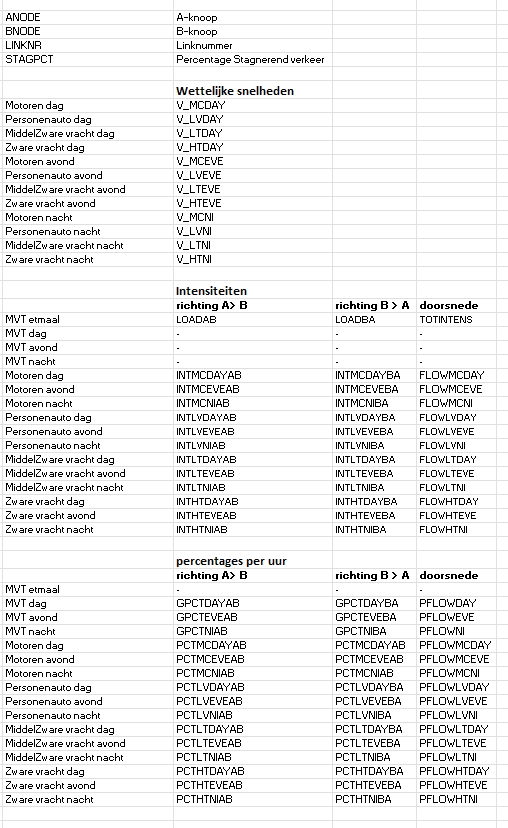
\includegraphics[keepaspectratio]{Others/images/clipboard-3863380911.png}}

\section{Dagdeel Calculation Periods}\label{dagdeel-calculation-periods}

\begin{Shaded}
\begin{Highlighting}[]
\NormalTok{DAY }\SpecialCharTok{=\textgreater{}}\NormalTok{ dag }\OtherTok{=} \DecValTok{12}\NormalTok{ uur}
\NormalTok{EVE }\SpecialCharTok{=\textgreater{}}\NormalTok{ avond }\OtherTok{=} \DecValTok{4}\NormalTok{ uur}
\NormalTok{NI }\SpecialCharTok{=\textgreater{}}\NormalTok{ nacht }\OtherTok{=} \DecValTok{8}\NormalTok{ uur}

\NormalTok{Rekenvoorbeeld}
\NormalTok{Dag LV }\SpecialCharTok{*} \DecValTok{12} \SpecialCharTok{+}\NormalTok{ Avond LV }\SpecialCharTok{*} \DecValTok{4} \SpecialCharTok{+}\NormalTok{ Nacht LV }\SpecialCharTok{*} \DecValTok{8} \SpecialCharTok{=\textgreater{}}\NormalTok{ LV Etmaal}
\end{Highlighting}
\end{Shaded}

\part{Prototype4}

\chapter*{Why?}\label{why}
\addcontentsline{toc}{chapter}{Why?}

\markboth{Why?}{Why?}

This model takes a shift from trip-based model to a tour based model.

\section*{Process-Flowchart}\label{process-flowchart}
\addcontentsline{toc}{section}{Process-Flowchart}

\markright{Process-Flowchart}

\chapter{Modules}\label{modules}

\section{CARMOD Module}\label{carmod-module}

\subsection{Purpose}

Its primary function is to ensure that the car ownership (autobezit)
within the Model is consistent with the car ownership totals provided by
the DYNAMO model. Additionally, CARMOD is responsible for spatially
distributing this car ownership.

\subsection{Inputs}

Following are the inputs to this job.

\begin{Shaded}
\begin{Highlighting}[]
\NormalTok{fratarTest}\AttributeTok{.source\_cube} \OperatorTok{=} \VerbatimStringTok{\textquotesingle{}2020\_KAL\textquotesingle{}} \CommentTok{\# Geef MatrixCube op (hier: 2016\_SMC)        }
\NormalTok{fratarTest}\AttributeTok{.matrix} \OperatorTok{=} \KeywordTok{[}\DecValTok{1}\NormalTok{,}\DecValTok{2}\NormalTok{,}\DecValTok{1}\NormalTok{,}\DecValTok{103}\KeywordTok{]}     \CommentTok{\# Geef Matrix (1 PER AANROEP!) (Hier Auto OS)}
\end{Highlighting}
\end{Shaded}

\subsection{.coeff File}

This file contains the updated Alternative Specific Constants (ASCs) and
other coefficients for the autobezit model, which are used by the SES
program

See Online Version for a sample .coeff file.

\subsection{.sum File}

Download the code.\href{../../first.rb}{matrixcompress.rb}

\subsection{.log File}

\section{QUAD}\label{quad}

\subsection{Purpose}

Some text explaining what the code does.

\subsection{Inputs}

Following are the inputs to this job.

\subsection{Outputs}

Following are the outputs to this job.

\subsection{Code}

Download the code.\href{../first.rb}{matrixcompress.rb}

\section{IntraLOS}\label{intralos}

\subsection{Purpose}

Some text explaining what the code does.

\subsection{Inputs}

Following are the inputs to this job.

\subsection{Outputs}

Following are the outputs to this job.

\subsection{Code}

Download the code.\href{../first.rb}{matrixcompress.rb}




\end{document}
